\section{Analysis of a Simple System Observable}

An Elementary Cellular Automaton with $n$ sites per time step has
$n$ degrees of freedom.
As one studies ECAs with larger $n$ values, it becomes a daunting
task to track the state of each individual site at each time step, and
an analysis of the time evolution of the system as a whole becomes
more meaningful.
In order to study the general behavior of the ECA systems, we wanted
to define an observable which collapsed these $n$ degrees of freedom
into one number whose value could be tracked over many time steps.
However, there are only so many such variables for such simple
systems value is meaningful for a wide variety of initial conditions
and boundary condition constraints.


\subsection{Defining an Observable}

We chose to study the density of black blocks as a convenient
observable for collapsing the information encoded in an $n$-site ECA
into one value per time step.
For ECAs with periodic or fixed boundary conditions, the density of
black blocks is straightforward:

\begin{equation}
    \rho = \frac{n_{black}}{n},
\end{equation}

\noindent where $n$ is the number of sites in the ECA.

One must be careful in the case of ECAs without boundary conditions
because the extent of the ECA is essentially infinite, and the above
definition of the black block density is not well-defined.
However, because the ECA rules only allow the state of a block to
depend on the previous states of its immediate neighbors, we chose
an initial condition of one black block surrounded by an infinite
number of white blocks on either side and constrained our studies to
rules which allow black blocks to spread by only one site per time
step.
Under these conditions there can be no black blocks outside of the
triangle with width $w(t)$ defined by $w(t) = 2t+1$, where $t$ is the
number of time steps since the initial state.
Treating $2t+1$ as the effective size of the Cellular Automaton at a
given time, the density of black blocks can be redefined as

\begin{equation}
    \rho = \frac{n_{black}}{(2t+1)}.
\end{equation}

\subsection{Density Time Evolution}
For ECAs with periodic or fixed boundary conditions, there is a
maximum number of global states available to the system: if there are
$n$ sites and each must have a value of 0 or 1, there will be $2^n$
possible states.
As such, after at most $2^n$ time steps the system must return to
a state that it has visited previously, and of course the density as a
function of time will be periodic.

However, ECAs with no boundaries have access to an infinite number of
states and therefore can exhibit a much richer density spectrum.
Any observed periodic behavior is significant because the system is
not confined to a finite number of states, and periodicity in the
density can only come about due to the intrinsic properties of a
particular rule.
Because of this, we have chosen to present the density's time
evolution for infinite ECAs.

Clearly not all ECA rules are created equally, and several of them are
not suitable for a study such as this.
For instance, with an initial state of one black block the Cellular
Automaton governed by rule 254 (Figure~\ref{rule254}) yields a string
of black blocks with width $2t+1$ at time step $t$.
This ECA will have a constant black block density of 1 given the above
definition.
However, most rules yield an interesting time evolution.
We will focus on the two rules mentioned previously, one (rule 126) of which is
very clearly periodic and has a well-defined structure and one (rule
30) whose dynamics appear to be random and incoherent.
The density as a function of time for rule 126 can be found in
Figure~\ref{126density}; that for rule 30 can be found in
Figure~\ref{30density}.


\begin{figure}
    \begin{minipage}[b]{0.49\textwidth}
        \centering
        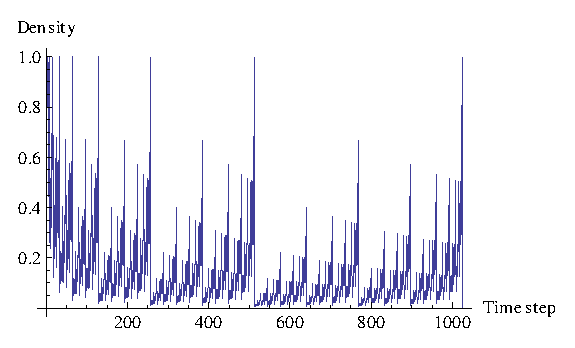
\includegraphics[width=\textwidth]{126density.eps}
        \caption{\label{126density} The black block density of rule 126 plotted as a function of time step}
    \end{minipage}
    \hspace{0.5cm}
    \begin{minipage}[b]{0.49\textwidth}
        \centering
        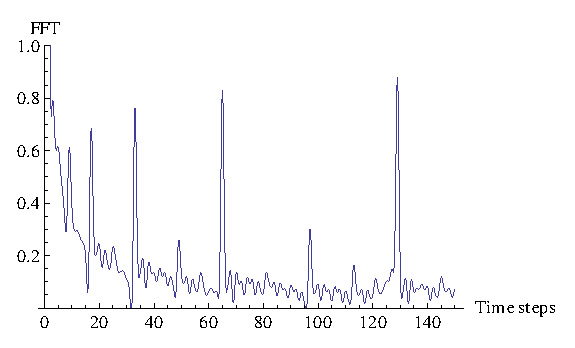
\includegraphics[width=\textwidth]{126FFT.eps}
        \caption{\label{126FFT} The Fast Fourier Transform (FFT) of
        rule 126's black block density, showing sharp peaks at 2$^n$}
    \end{minipage}
\end{figure}


\begin{figure}
    \begin{minipage}[b]{0.49\textwidth}
        \centering
        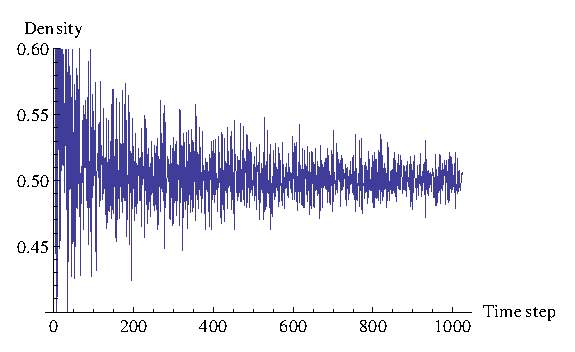
\includegraphics[width=\textwidth]{30density.eps}
        \caption{\label{30density} The black block density of rule 30 plotted as a function of time step}
    \end{minipage}
    \hspace{0.5cm}
    \begin{minipage}[b]{0.49\textwidth}
        \centering
        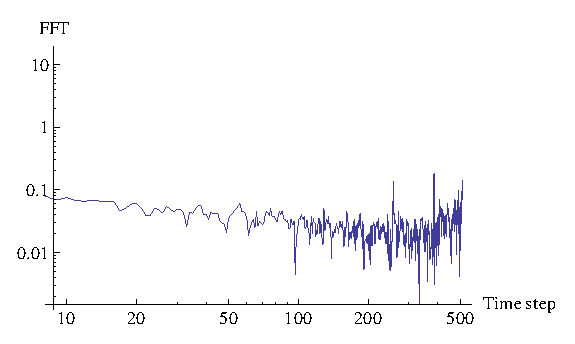
\includegraphics[width=\textwidth]{30FFT.eps}
        \caption{\label{30FFT} The FFT of rule 30's black block density}
    \end{minipage}
\end{figure}


\subsection{Periodic Density Analysis}
In order to establish whether or not an ECA's black block density
exhibits periodicity, we chose to look at its Discrete Fourier
Transform (DFT), specifically the Fast Fourier Transform (FFT), as
well as its Autocorrelation.

The DFT of a sequence of values is defined as

\begin{equation}
    \rho_p = \sum_{t=0}^{T-1} \rho_t e^{-2\pi i pt/T} \qquad p =
    0, 1,\ \ldots\ T,
\end{equation}

\noindent where $\rho_t$ is the black block density at a time step
$t$, $T$ is the total number of time steps, and $p$ is an integer
value of time steps which labels the discrete frequency
$\omega_p = p/T$.
Values of $p$ with a high coefficient $\rho_p$ correspond to strong
sinusoidal motion with a frequency of $\omega_p$.

From Figure~\ref{126FFT} we can see that rule 126 has clear sinusoidal
behavior, especially for values of $p$ that are a power of 2 ($2^n$
with integer $n$).
This is not terribly surprising given the structure of the ECA under
rule 126 in Figure~\ref{rule126}.

However, Figure~\ref{30FFT} shows that the opposite is true for rule
30.
In fact, the density FFT for rule 30 closely resembles that of random
noise, which should have a flat response as a function of frequency.

Similarly, the Autocorrelation function of a sequence of real values
is given by

\begin{equation}
    C_\tau = \frac{1}{T}\sum_{t=0}^{T-1} \rho_t \ \rho_{t-\tau} \qquad
    \tau = 0, 1,\ \ldots\ T,
\end{equation}

\noindent where $\rho_t$ is the black block density at a time step
$t$, $T$ is the total number of time steps, and $\tau$ is an integer
value of separation in time.
A high coefficient $C_\tau$ corresponds to a time separation for which
the density of black blocks is strongly correlated.
For example, a large value of $C_5$ would suggest that densities
separated by 5 time steps tend to have approximately the same value,
while a coefficient close to zero implies that they fluctuate randomly
around the mean.
If they are anticorrelated, we would see a negative autocorrelation
coefficient.

\begin{figure}
    \begin{minipage}[b]{0.49\textwidth}
        \centering
        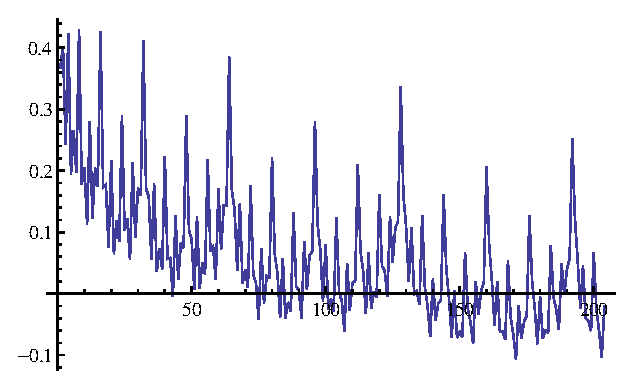
\includegraphics[width=\textwidth]{126corr.eps}
        \caption{\label{126corr} The black block density's
        Autocorrelation for a rule 126 ECA.}
    \end{minipage}
    \hspace{0.5cm}
    \begin{minipage}[b]{0.49\textwidth}
        \centering
        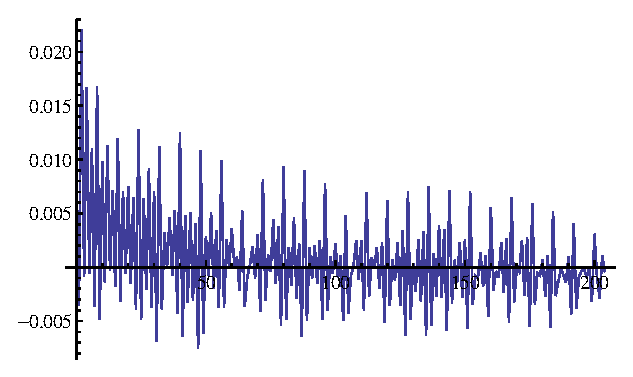
\includegraphics[width=\textwidth]{30corr.eps}
        \caption{\label{30corr} The black block density's
        Autocorrelation for a rule 30 ECA.}
    \end{minipage}
\end{figure}

Figure~\ref{126corr} shows that there is a strong correlation between
densities separated by a time period equal to a power of 2.
Again, this is not unexpected given the structure rule 126 imposes and
the sinusoidal features expressed in its DFT.
Furthermore, the correlation is non-zero at short time scales ($<50$ time steps) 
but averages to zero over longer time scales.  



Figure~\ref{30corr}, however, has some very interesting features which
lend a little more insight to rule 30 than its density DFT.
Despite what appears to be random behavior, there are clear correlations
between densities separated by 8 time steps.
This is in part be due to the quasi-periodic behavior of the left
half of rule 30's ECA (see Figure~\ref{rule30}).
However, the fact that this correlation is also present for time
separations that are multiples of 8 suggests that its right half
(which seems to be without structure) is not as random as at first
glance.
The short term autocorrelation of rule 30, which is approximately zero,
contrasts with that of rule 126, which is positive at short time scales.
